\documentclass{report}

\usepackage[utf8]{inputenc}
\usepackage{graphicx}
\usepackage[margin=35mm]{geometry}
\usepackage[colorlinks = true,linkcolor = red, urlcolor  = blue, citecolor = blue, anchorcolor = blue]{hyperref}
\usepackage[pagestyles]{titlesec}
% Load the package with the acronym option
\usepackage[automake]{glossaries}

 

\usepackage[backend=bibtex,style=numeric,sorting=none]{biblatex}


\addbibresource{bibresource.bib}  

\titleformat{\chapter}[display]
    {\normalfont\huge\bfseries}{\chaptertitlename\ \thechapter}{20pt}{\Huge}
\titlespacing*{\chapter}{0pt}{-30pt}{20pt}

\titleformat{\chapter}%
  {\normalfont\bfseries\LARGE}{\thechapter.}{10pt}{}

\titleformat{\section}%
  {\normalfont\bfseries\large}{\thesection.}{10pt}{}

\titleformat{\subsection}%
  {\normalfont\bfseries\small}{\thesubsection.}{10pt}{}

% Acronym definitions

\newacronym{DoS}{DoS}{Denial-of-service attack}
\newacronym{DDoS}{DDoS}{distributed denial-of-service attack}
\newacronym{OSI}{OSI}{Open Systems Interconnection}
\newacronym{SSL}{SSL}{Secure Sockets Layer}
\newacronym{TCP}{TCP}{Transmission Control Protocol}
\newacronym{ICMP}{ICMP}{Internet Control Message Protocol}
\newacronym{APDoS}{APDoS}{The advanced persistent denial-of-servicel}
\newacronym{SNMP}{SNMP}{Simple Network Management Protocol}
\newacronym{CDN}{CDN}{Content delivery network}
\newacronym{UDP}{UDP}{User Datagram Protocol}
\newacronym{IP}{IP}{Internet Protocol}
\newacronym{IPS}{IPS}{Intrusion Prevention System}
\newacronym{MAC}{MAC}{Media Access Control}
\newacronym{ISP}{ISP}{Internet Service Providerl}
\newacronym{SDN}{SDN}{Software-Defined Networking }

% Generate the glossary
\makeglossaries


\title{Automatically defend from DoS and DDoS traffic flood attacks}
\author{Yinon Cohen and Maor Shabtay\\\\{ Advisor: Dr. Amit Dvir}\\\\{Ariel University}}

\date{October 2017}

\begin{document}
\maketitle

\tableofcontents
\addtocontents{toc}{~\hfill\textbf{Page}\par}


\newpage

\chapter {Abstract}
\hfill \break \gls{DoS} and \gls{DDoS} attacks are attempts to exhaust server side assets, and designed to prevent client-to-server communication (denial of service). These attacks aim to both public and private sectors, and occur more and more frequently. In addition, lately the massive \gls{DDoS} attacks are performing 100 Gigabits per second, and being more common than ever. These attacks are sowing fear among organizations and private server owners.

\hfill \break Our project deals with understanding and examining \gls{DoS} and \gls{DDoS} attacks, and what are the solutions for them. In particularly, we will discuss and handle with traffic flood attacks on web servers, and will try to develop our own software or algorithm to block or to give any immediately pragmatic solution.

\hfill \break Our main goal is to develop an automatic system that would identify and analyze a traffic flood attack, defend the server from it, and in need - will block any \gls{IP} or sub-net which the flood comes from. Our system should run on a \gls{CDN} instead of on the server in order to save the server’s performances providing service
\hfill \break \hfill \break
    \begin{center}
        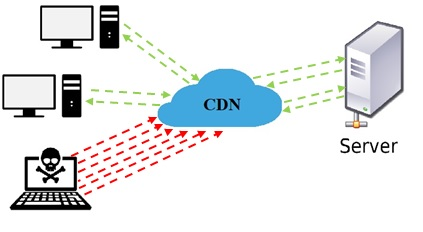
\includegraphics{pi}
    \end{center}
\newpage
\chapter {Introduction}
\section {DoS}
\hfill \break \gls{DoS} attacks are attempts to exhaust server-side assets and designed to prevent client-to-server communication (denial of service). Simply, we can say that stealth server sabotage wires or even the server is denial of service, but in the context of data security we discuss about remote attacks and not physical sabotaging.
\section {DDoS}
\hfill \break \gls{DDoS} attacks are very similar and sometimes even identical, and their intention is Distributed Denial of Service. In other words, the attack comes not from a single source, but from a large number of end stations – usually triggered by the attacker in the form of a king of virus located on these end stations. Most \gls{DDoS} attacks are much more powerful and significant. It is important to understand that even an attack by two or three end stations is usually considered as a \gls{DoS} attack, since there is really no significant flooding of the server.
\hfill \break Earlier this month Cisco released a white paper that \cite{corero} is part of the company’s larger report, “Visual Networking Index Complete Forecast Update, 2015-2020.” Here are some statistics from that white paper, relevant to distributed denial of service (\gls{DDoS}) attacks:
\begin{itemize}
\item Frequency of distributed denial-of-service (\gls{DDoS}) attacks has increased more than 2.5 times over the last 3 years.
\item	The average size of \gls{DDoS} attacks is increasing steadily and approaching 1 Gbps, enough to take most organizations completely off line.
\item	Peak \gls{DDoS} attack size (Gbps) is increasing in a linear trajectory, with peak attacks reaching 300, 400, and 500 Gbps respectively, in 2013, 2014, and 2015, at about 10 to 15 percent per year.
\item	In 2015 the top motivation behind \gls{DDoS} attacks was criminals demonstrating attack capabilities, with gaming and criminal extortion attempts in second and third place, respectively.
\item	\gls{DDoS} attacks account for more than 5 percent of all monthly gaming-related traffic and more than 30 percent of gaming traffic while they are occurring.
\item	Globally the number of \gls{DDoS} attacks grew 25 percent in 2015 and will increase 2.6-fold to 17 million by 2020.
\end{itemize}

\hfill \break The \gls{DoS} and \gls{DDoS} attacks can be divided into two types: 
\begin{itemize}
\item 	Attacks that flood and delay the service.
\item	Attacks that completely disrupt the service (and these we want to deal with in our project).

\end{itemize}
\begin{figure}
  \centering
        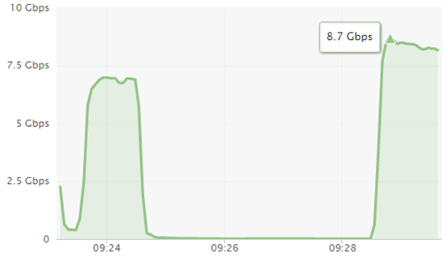
\includegraphics{ddos-attack-traffic-gbps}
	\caption{Sudden increase in server network traffic}
    \end{figure}

\section{DoS and DDoS attacks}
Our research is including both types of attacks for \gls{DoS} and \gls{DDoS} attacks in general, and we will divide the types into different main types, based on the seven-layer-model (\gls{OSI}) \cite{QuickGuide}.
\subsection {DoS and DDoS over Application layer} 
 \hfill \break Attacks in the application layer are often generated by POST requests. They are also divided to sub protocols in the application layer – http / https.
\begin{itemize}
\item\underline {HTTP POST Flood} 
- Creating and sending very large number of POST methods, to the extent that the server can't answer all requests, therefore service for real users of the server is compromised.

\item\underline{HTTPS POST Flood} - This is a flood of post methods that pass through \gls{SSL} Session. The purpose of \gls{SSL} is to take every message and decrypt it in order to inspect it. Flooding of these methods would harm the service.
\newpage
\item\underline{HTTP GET Flood} - The attacker creates and sends to the server a huge amount of GET requests. The server needs to analyze all of them and return some data. Some people regard this attack as a Transport-layer attack, since sometimes the server would have to send a lot of data to the user attacker. Therefore, traffic and network bandwidth are flooded. Denial and service prevention depends on the server’s capacity to getting and sending back packets. If it is able to handle a huge number of requests – the traffic will be damaged, and if it fails, the requests that it receives from real users will not be handled as the server falls.

\item\underline{HTTPS GET Flood} - Overflow of GET requests on HTTPS protocol requires a lot of work from \gls{SSL} Session – decryption every message and hence load and sabotage the service.
\end{itemize}
\hfill \break
\subsection {DoS and DDoS over Transport layer} 

 Flooding over Transport layer characterized mainly by packets that the server receives and is required to provide service – mostly by sending a requested data or any other response\cite{QuickGuide}.\begin{itemize}
 \item\underline{Syn Flood} - In this attack, the attacker takes advantage of the \gls{TCP} principles that the server always wants to reach. When a server receives a Syn packet, it is a request from a client to open a connection, and it is obligated to respond to it and must return the client a Syn – Ack certificate. Each Syn message requires time from the server – analyzing the packet (understanding who created it, calculating ‘Check-sum’ etc.), and then be able to reply. Therefore, flooding these messages is slowing down and compromising the server’s serviceability.

\item\underline{Rst Flood} - Like Syn flood, the attacker takes advantage of \gls{TCP} principles, including reliable communication. In case that a socket is closed or when one of the sides disconnected (and in few other situations), \gls{TCP} has a solution. The connected side still wants to continue the communication (since there was no closing connection process), it sends a packet with a Rst flag and hence they have to re-open the connection. Like Syn packets overflowing, Rst packets overflowing also require a lot of work from the server and would sabotage the service.

\item\underline{\gls{UDP} Flood} - \gls{UDP} floods are used frequently for larger bandwidth \gls{DDoS} attacks because they are connectionless and it is easy to generate \gls{UDP} messages from many different scripting and compiled languages. The attack can be initiated by sending a large number of \gls{UDP} packets to random ports. As a result, the server would check for the application listening at that port, realize that no one is and reply with \gls{ICMP} packet saying ‘Destination Unreachable’. Thus, for a large number of \gls{UDP} packets, the server will be forced into sending many \gls{ICMP} packets and much performance.
\end{itemize}
\newpage
\subsection {DoS and DDoS over Network layer} 

 \hfill \break \gls{DoS} and \gls{DDoS} attacks over the Network layer are characterized with a large number of packets in order to overload the bandwidth and exhaust network resources. Network resources can be routers, firewalls and servers, and it is clear that their ability is final.
\begin{itemize}
\item\underline{\gls{ICMP} Flood} - \gls{ICMP} protocol is typically used for error messages rather than data exchange between systems. Flooding messages with \gls{ICMP} protocol – e.g. ping – is intended to overload the network.
\end{itemize}
 \hfill \break
\subsection {DoS and DDoS over Link layer}  

 \hfill \break \gls{DoS} and \gls{DDoS} attacks over the Network layer require access to the local network. Therefore, they are rare and more easy to detect.
\begin{itemize}
\item\underline{\gls{MAC} Flood} - A rare attack, in which the attacker has to be connected to the local switch. The attacker sends multiple dummy Ethernet frames, each with different invalid \gls{MAC} address. Network switches maintaining their \gls{MAC} table, and treating \gls{MAC} addresses separately, and hence reserve some resources for each request. When all the memory in the table is used up, it either shuts down or becomes unresponsive.
\end{itemize}


 \hfill \break
\subsection {Demonstrating APDoS Attack}

 \hfill \break  \gls{APDoS} is an attack that combines many \gls{DoS} and \gls{DDoS} attacks, and is carried out by a lot of hostile elements over time. \gls{APDoS} represents the worst Denial of Service attack that can occur. The idea behind it is a combination of many attacks from multiple endpoints, and over long period of time, hence its name Advances Persistent \gls{DoS}. In this attack, the attackers usually attack several stations in order to create a distraction from the \gls{DoS} defenses, but concentrate on one main victim in the organization.
\newpage
\section{DoS and DDoS defense solutions }

\subsection{DoS and DDoS solutions over Application layer}
 
\begin{itemize}
\item\underline {HTTP POST Flood} -  There is a difficulty in distinguishing between legal traffic and attack.
The most effective mechanism that exists today is by combining methods of characterizing the movement of requests and identifying the source user.
When a random url is used, an exception check is required to understand that this was an attack and not an innocent use of the server \cite{AppstSolution}. Part of the exception check is to try to identify the source user that triggers the attack, and you may notice that sometimes a large part of the package signature and content is the same.

\item\underline {HTTPS Request Flood} - Using the BIG-IP system \cite{HTTPSRequestSolution} and the F5 iRules scripting language.
Now available via the F5 DevCentral online community, this iRule states that if a device tries to renegotiate more than five times in any 60-second period, the connection is silently dropped.
The biggest benefit to this approach is that the attacker believes the attack is still working and in service, when in actuality, the server has ignored the request and moved on to processing valid user requests instead.


\item\underline {HTTP GET Flood} Today We know about two detection algorithms \cite{AppstSolution}, one is focusing on a browsing order of pages and the other is focusing on a correlation with browsing time to page information size. that implement detection techniques and evaluate attack detection rates, i.e., false positive and false negative. The results show that our techniques can detect the HTTP-GET flood attack effectively.
\end{itemize}

\subsection {DoS and DDoS solutions over Transport layer} 
\begin{itemize}
\item\underline{Syn Flood} - We have a lot of solution \cite{SynSolution} for this attack:
Filtering ,Increasing Backlog,Reducing SYN-RECEIVED Timer,Recycling the Oldest Half-Open \gls{TCP},SYN Cache,SYN cookies,Hybrid Approaches,Firewalls and Proxies
We will expand a bit on SYN cookie is a technique used to resist SYN flood attacks. The technique's primary inventor Daniel J. Bernstein defines SYN cookies as "particular choices of initial \gls{TCP} sequence numbers by \gls{TCP} servers." In particular, the use of SYN cookies allows a server to avoid dropping connections when the SYN queue fills up. Instead, the server behaves as if the SYN queue had been enlarged. The server sends back the appropriate SYN+ACK response to the client but discards the SYN queue entry. If the server then receives a subsequent ACK response from the client, the server is able to reconstruct the SYN queue entry using information encoded in the \gls{TCP} sequence number.

\item\underline {Rst Flood} - A RST packet is accepted if the sequence number is in the receiver's window, or when a connection is closed (closed socket). This is slightly different from a FIN, which just says that the other endpoint will no longer be transmitting any new data but can still receive some.

There are three types of event that cause a RST to be emitted. A) the connection is explicitly aborted by the endpoint, e.g. the process holding the socket being killed (just closing the socket normally is not grounds for RST, even if there is still unreceived data). B) the \gls{TCP} stack receiving certain kinds of invalid packets, e.g. a non-RST packet for a connection that doesn't exist or has already been closed. C) An unexpected amount of RST packets gained and there is no stopping point when sending back even a few responses.
Emmiting these senarios would mitigate the performance and engagement of the server with unwanted traffic. \cite{RstSolution}.
\end{itemize}

\subsection {DoS and DDoS solutions over Network layer} 
\begin{itemize}
\item\underline {\gls{ICMP} Flood} - Reconfiguring your perimeter firewall to disallow pings will block attacks originating from outside your network, albeit not internal attacks \cite{ICMPSolution}. Still, the blanket blocking of ping requests can have unintended consequences, including the inability to diagnose server issues.
The Incapsula \gls{DDoS} protection provide blanket protection against \gls{ICMP} floods by limiting the size of ping requests as well as the rate at which they can be accepted.
\end{itemize}
 \hfill \break

\subsection {APDoS solution}

 \hfill \break To combat \gls{APDoS}, organizations require a single vendor, hybrid cyber security solution that protects networks and applications from a wide range of attacks. Ideally, such a solution \cite{APDoSSolution} includes all the different technologies needed for effective detection and mitigation, including \gls{DoS}/\gls{DDoS} protection, behavioral analysis, \gls{IPS}, encrypted attack protection and web application firewall (WAF). Additionally, organizations also require new levels of partnership with their \gls{DDoS} mitigation service provider and any \gls{ISP} that provides managed \gls{DDoS} services to coordinate for the effective detection and mitigation of a multi-vector assault.

\newpage
\chapter {Related Work}
\section {Related Articles}
\subsection {Traffic flooding attack detection with SNMP MIB using SVM}
\gls{DoS} and \gls{DDoS} attacks have become more and more destructive, and are threatening to various network services. Hence, the various methods of protection and monitoring and control of network traffic have also begun.
However, most of the current modern detection systems are focusing on detail analysing for each packet’s data, which causes late detection and can’t handle high network traffic.
  \hfill \break
 \gls{SNMP}\cite{snmp}  provides a universal method of exchanging data for purposes of monitoring systems that reside on a network. The use of  \gls{SNMP} is most dominant in the modern industry. But, to utilize  \gls{SNMP} for traffic flooding attack detection, we need to consider the following three points in the use of the  \gls{SNMP} MIB variables which affects the performance and accuracy of the detection system:
\begin{itemize}
\item Proper selection of  \gls{SNMP} MIB variables for attack detection
\item Determination of the detection timing about when and how often
\item Algorithm for attack detection using the selected MIB (Management Information Base) variables.
\end{itemize}
  \hfill \break

\subsection {Change trend of averaged Hurst parameter of traffic under DDoS flood attacks}
\gls{DoS} and \gls{DDoS} flood attacks are great threats to the internet though various approaches and systems have been proposed. Hence, Intrusion Detecting System (IDS) and Intrusion Preventing System (\gls{IPS}) are desired. The \gls{DDoS} flood attack sends packets upon a server with a huge amount of traffic. It never tries to break into the server’s system, which makes the servers’s security defenses irrelevant.
\hfill \break
The solutions given by misuse detection are primarily based on a library of known signatures to match against network traffic . Hence, unknown signatures from new variants of an attack mean are hard to be recognized. Therefore, anomaly detectors (exceeded routine detectors) play a role in detection of \gls{DDoS} flood attacks.
\hfill \break
It is important considering the Hurst parameter - H in characterizing exceptions of traffic series in packet size under DDOS flood attacks. This paper specifically  \cite{Hurst} studies how H of traffic is changing under \gls{DDoS} flood attacks. It it important understanding the following:
\begin{enumerate}
\item Whether H of traffic when a server is under \gls{DDoS} flood attacks is much different from the regular one?
\item How is H changes when a server suffers from \gls{DDoS} flood attacks?
\end{enumerate}
Answering these questions might give us better understanding for detecting and protecting from \gls{DDoS} flood attacks.
\hfill \break

\subsection{Software-Defined Networking (SDN) and Distributed Denial of Service (DDoS) Attacks in Cloud Computing Environments }
Cloud computing develops rapidly due to its essential characteristics. Cloud computing would not be possible without the underneath support of networking. Recently, \gls{SDN}  \cite{SDN} has attracted great interests as a new paradigm in networking. In \gls{SDN} , network intelligence and state are logically centralized, and the underlying network infrastructure is abstracted from the applications. Denial of Service (\gls{DoS}) attacks and Distributed De-
nial of Service(\gls{DDoS}) flooding attacks are the main methods to destroy availability of cloud computing.
Although the capabilities of \gls{SDN}  make it easy to detect and to react\gls{DDoS} attacks in cloud environments, the separation of the control plane from the data plane in \gls{SDN}  introduces new attack planes. \gls{SDN}  itself may be a target of some attacks, and potential \gls{DDoS} vulnerabilities exist across \gls{SDN}  platforms. For example, an attacker can take advantages of the characteristics of \gls{SDN}  to launch \gls{DDoS} attacks against the control layer, infrastructure layer plane and application layer of \gls{SDN} .
 \hfill \break
\section {Related Productions}
\subsection {Cisco - 'DDoS Mitigation' } 
Cisco had developed a System which delivers a complete \gls{DDoS} protection solution based on the principles of detection, diversion, verification, and forwarding to help ensure total protection\cite{cisco}. The solution maintains the business continuity by: 
\begin{itemize}
\item Detecting the \gls{DDoS} attack.
\item Diverting  the data traffic destined for the target device to  a Cisco appliance for treatment.
\item Analyzing and filtering  the bad traffic flows from the good traffic flows packets, preventing malicious traffic from impacting performance while allowing legitimate transactions to complete.
\item Forwarding  the good traffic to maintain business continuity.
\end{itemize}

\subsection {Check Point -  'DDoS Protector' }
Check Point had developed a System called '\gls{DDoS} Protector'\cite{checkpoint}, which keeps businesses running with multi-layered, customizable protections and up to 40Gbps performance that automatically defends against network flood and application layer attacks with fast response time against today’s sophisticated denial of service attacks.
\hfill \break
\gls{DDoS} Protector Appliances offer flexible deployment options to easily protect any size business, and integrated security management for real-time traffic analysis and threat management intelligence for advanced protection against\gls{DDoS} attacks.
The product provides multi-layer protections, handles network and traffic flood and has a management system.
  \hfill \break

%Print the glossary
\printglossary[type=\acronymtype,title=Abbreviations]
\newpage
\addcontentsline{toc}{chapter}{References}
\printbibliography[title=References]

\end{document}
